% HumanBench v0.1 paper, first full draft.
% Build: tectonic --keep-intermediates humanbench.tex (see paper/README.md).
% Every number is traced to a repository file in paper/README.md; the data figures are made by
% paper/figures/make_figures.py.
\documentclass[10pt,twocolumn]{article}

\usepackage{iftex}
\ifPDFTeX
  \usepackage[T1]{fontenc}
  \usepackage[utf8]{inputenc}
  \usepackage{lmodern}
\fi
\usepackage[letterpaper,margin=0.7in,columnsep=0.25in]{geometry}
\usepackage{amsmath}
\usepackage{graphicx}
\usepackage{booktabs}
\usepackage{array}
\usepackage{xcolor}
\usepackage[numbers,sort&compress]{natbib}
\usepackage{tikz}
\usetikzlibrary{positioning,arrows.meta,calc}
\usepackage[font=small,labelfont=bf,labelsep=period,skip=5pt]{caption}
\usepackage[colorlinks=true,linkcolor=black,citecolor=blue!50!black,urlcolor=blue!50!black]{hyperref}

\setlength{\emergencystretch}{2em}
\renewcommand{\bibfont}{\footnotesize}
\setlength{\bibsep}{1.5pt}
\setlength{\parskip}{0pt plus 1.2pt}
\frenchspacing
\renewcommand{\topfraction}{0.95}
\renewcommand{\bottomfraction}{0.9}
\renewcommand{\textfraction}{0.05}
\renewcommand{\floatpagefraction}{0.85}
\renewcommand{\dbltopfraction}{0.95}
\renewcommand{\dblfloatpagefraction}{0.85}
\setcounter{topnumber}{3}
\setcounter{dbltopnumber}{3}
\setlength{\textfloatsep}{11pt plus 3pt minus 2pt}
\setlength{\dbltextfloatsep}{11pt plus 3pt minus 2pt}
\setlength{\floatsep}{9pt plus 2pt minus 2pt}
\setlength{\dblfloatsep}{9pt plus 2pt minus 2pt}
\makeatletter
\renewcommand\section{\@startsection{section}{1}{\z@}{-2.6ex \@plus -1ex \@minus -.2ex}{1.5ex \@plus .2ex}{\normalfont\Large\bfseries\raggedright}}
\renewcommand\subsection{\@startsection{subsection}{2}{\z@}{-2.3ex \@plus -.8ex \@minus -.2ex}{1.1ex \@plus .2ex}{\normalfont\large\bfseries\raggedright}}
\renewcommand\paragraph{\@startsection{paragraph}{4}{\z@}{1.5ex \@plus .6ex \@minus .2ex}{-1em}{\normalfont\normalsize\bfseries}}
\makeatother

% Where the benchmark lives. The website and repository addresses are defined below.
\newcommand{\hbrepo}{https://github.com/pragnyanramtha/human-bench}
\newcommand{\hbsite}{https://humanbench.agent7.dev}
\makeatletter
\edef\hb@repo{\hbrepo}\edef\hb@site{\hbsite}
\newcommand{\hbrepourl}{\expandafter\url\expandafter{\hb@repo}}
\newcommand{\hbsiteurl}{\expandafter\url\expandafter{\hb@site}}
% Tables keep the model identifiers in the source (paper/check_numbers.py reads them) and print display names.
\newcommand{\mdl}[1]{\@ifundefined{hbname@#1}{\texttt{#1}}{\@nameuse{hbname@#1}}}
\@namedef{hbname@claude-fable-5-2}{Claude Fable 5.2}
\@namedef{hbname@claude-opus-5-5}{Claude Opus 5.5}
\@namedef{hbname@claude-sonnet-5-5}{Claude Sonnet 5.5}
\@namedef{hbname@claude-haiku-5-5}{Claude Haiku 5.5}
\@namedef{hbname@gpt-6.1-sol}{GPT-6.1 Sol}
\@namedef{hbname@gpt-6.1-terra}{GPT-6.1 Terra}
\@namedef{hbname@gpt-6-astra}{GPT-6 Astra}
\@namedef{hbname@gpt-6-luna}{GPT-6 Luna}
\@namedef{hbname@deepseek-v4p1-flash-1017}{DeepSeek V4.1 Flash}
\@namedef{hbname@kimi-k3p1-pro}{Kimi K3.1 Pro}
\@namedef{hbname@minimax-m3p1-flash}{MiniMax M3.1 Flash}
\makeatother
\newcommand{\code}[1]{\texttt{#1}}
\newcommand{\hb}{HumanBench}
% One palette for every figure (the same values as paper/figures/make_figures.py).
\definecolor{hbpassed}{HTML}{274FA3}  % ink blue: passed
\definecolor{hbflagged}{HTML}{C4710F} % amber: flagged as AI
\definecolor{hbquality}{HTML}{50555C} % dark grey: rejected by judge
\definecolor{hbchecks}{HTML}{B3B7BD}  % light grey: failed checks

\title{\LARGE\textbf{HumanBench: Can AI Write Like a Human?}}
\author{Pragnyan Ramtha\\ \texttt{pragnyanramtha@agent7.dev}}
\date{}

\raggedbottom
\begin{document}
\maketitle

\begin{abstract}
\hb{} v0.1 gives models everyday writing tasks and puts each output through programmatic checks, an LLM judge and an AI-text detector. The HumanBench score is the share passing all three: the mean over three samples per task, then over all 212 tasks, with bootstrap intervals over tasks. Public and held-out scores are reported beside it. There are 132 public tasks (52 human-reference and 80 synthetic) and 80 held-out synthetic tasks. Across eleven models, scores range from 1.9\% to 23.1\%. Answer quality, the share passing the first two gates, ranges from 27.0\% to 83.3\%. HumanBench measures task compliance, a model-judged quality bar and detectability under named open AI-text detectors; no human readers were involved. Results depend on the detector, task mix, reasoning effort and model access, and models under test helped draft, audit and judge the benchmark. Public tasks, code and a text-free ledger are at \hbrepourl; results are at \hbsiteurl.
\end{abstract}

\section{Introduction}

People ask language models to write text that they will send under their own name: an email to a supplier, a reply in a forum thread, a product review, a toast, a postmortem. Two properties matter for this use. The text has to do the job that was asked. The text should also not be marked as machine-written by the AI-text detectors that are now run on such text. \hb{} v0.1 measures both properties on the same outputs.

\begin{figure*}[t]
\centering
\begin{tikzpicture}[x=1mm, y=1mm, font={\small\hyphenpenalty=10000 \exhyphenpenalty=10000 }, >={Stealth[length=4.6pt,width=4pt]},
  frame/.style={draw=black!80, line width=0.5pt, rounded corners=1.5pt},
  txt/.style={anchor=north west, align=left, inner sep=0pt, text width=#1},
  flow/.style={->, line width=0.7pt, draw=black!85},
  feed/.style={black!65, line width=0.5pt, dash pattern=on 2pt off 1.5pt},
  key/.style={line width=3pt, line cap=butt},
  num/.style={circle, fill=black!85, text=white, font=\small\bfseries, inner sep=0pt, minimum size=4.4mm}]
% the task: hidden lists above, request and notes below
\begin{scope}
  \clip[rounded corners=1.5pt] (0,-11.5) rectangle (30,27);
  \fill[black!9] (0,9) rectangle (30,27);
\end{scope}
\draw[frame] (0,-11.5) rectangle (30,27);
\draw[black!80, line width=0.5pt] (0,9) -- (30,9);
\node[anchor=south west, inner sep=0pt] at (0,28.2) {\textbf{Task}};
\node[txt=27mm] at (1.7,25.2) {\textbf{Hidden lists}\\must include,\\must cover,\\must not reveal};
\node[txt=27mm] at (1.7,7.2) {\textbf{Request, notes}\\as a user would\\type them; all that\\the model sees};
% the model
\draw[frame] (34,-11.5) rectangle (53,9);
\node[txt=16mm] at (35.7,7.2) {\textbf{Model}\\three samples\\per task};
% three outputs
\foreach \d in {1.4,0.7,0} {\draw[black!80, line width=0.4pt, fill=white] (56+\d,-3.7+\d) rectangle (59.2+\d,0.7+\d);}
% the gates
\foreach \x/\n/\head/\body in {
  64/1/{Programmatic\\checks}/{length, format, required facts and leaks},
  99/2/{LLM judge}/{yes/no questions; any ``no'' fails},
  134/3/{AI-text detector}/{threshold: 99\% of human texts stay at or below}} {
  \draw[frame] (\x,-11.5) rectangle (\x+29,9);
  \node[txt=26mm] at (\x+1.7,7.2) {\textbf{\head}\\\body};
  \node[num] at (\x,9) {\n};
}
\node[frame, fill=hbpassed, text=white, inner sep=0pt, minimum width=12mm, minimum height=7mm] (ok) at (174,-1.5) {\shortstack{passed\\all three}};
% the flow
\draw[flow] (30,-1.5) -- (34,-1.5);
\draw[line width=0.7pt, draw=black!85] (53,-1.5) -- (56,-1.5);
\draw[flow] (60.6,-1.5) -- (64,-1.5);
\draw[flow] (93,-1.5) -- (99,-1.5);
\draw[flow] (128,-1.5) -- (134,-1.5);
\draw[flow] (163,-1.5) -- (ok.west);
% the hidden lists feed the first two gates
\draw[feed] (30,19) -- (113.5,19);
\draw[feed, ->] (78.5,19) -- (78.5,9.2);
\draw[feed, ->] (113.5,19) -- (113.5,9.2);
\node[anchor=south west, inner sep=0pt] at (34,20.2) {only the first two gates read the hidden lists};
% the three ways to stop
\foreach \x/\c/\name in {78.5/hbchecks/{failed checks}, 113.5/hbquality/{rejected by judge}, 148.5/hbflagged/{flagged as AI}} {
  \draw[flow] (\x,-11.5) -- (\x,-16.7);
  \draw[key, \c] (\x-6,-18.4) -- (\x+6,-18.4);
  \node[anchor=north, inner sep=0pt] at (\x,-20.2) {\name};
}
\node[txt=60mm] at (0,-15.7) {\textbf{\hb{} score:} the share of a model's outputs that passed.};
\end{tikzpicture}
\caption{The protocol. A task holds a request and notes, which the model sees, and hidden lists, which only the first two gates read. The model produces three samples per task, and each output goes through the gates in order and stops at the first it fails. Look at the four endings: every output has exactly one outcome, and only an output that passes all three gates counts toward the score.}
\label{fig:protocol}
\end{figure*}

Existing evaluations cover the two properties separately. Detector benchmarks hold a set of texts fixed and score detectors on it \citep{dugan2024raid,li2023mage,wang2023m4,guo2023hc3}. They show how well a detector works. They do not show whether a given model can complete a writing task without being flagged, and a text can lower a detector's score by getting worse: the attacks studied in RAID include misspellings and character substitutions \citep{dugan2024raid}. Writing benchmarks score quality, preference or surface style with rubrics, model judges or pattern counts \citep{wu2025writingbench,fein2025litbench,roongta2026slopbench}. They do not ask whether an AI-text detector flags the text, and an output can satisfy a rubric while being written in a model's default style. Detectability alone can be raised by degraded text. A rubric alone mostly reports how well a model follows instructions.

\hb{} joins the two with a conjunction. Each task is stored in a \emph{card file}: a request as a user would type it, the user's notes, and hidden lists of what the output must contain, convey and keep out. A model produces three samples per task. Each output passes through three gates in order (Figure~\ref{fig:protocol}): programmatic checks, an LLM judge and an AI-text detector at a threshold that 99\% of a pool of human texts stay under. The \hb{} score is the share of outputs that pass all three. There are two kinds of task. A \emph{human-reference task} is built backwards from a real person's text, called the \emph{human reference}; that text passes the programmatic checks, is accepted by the main LLM judge and is not flagged by the headline detector. A \emph{synthetic task} has a model-written \emph{reference solution} that proves its checks can be met, and this kind also covers thread replies and simulated workspaces. The benchmark has 212 tasks. The 132 public tasks are 52 human-reference tasks and 80 synthetic tasks. The 80 held-out tasks are synthetic tasks that are held back. Every model gets one score over all tasks. Beside it, the public score lets anyone reproduce that part; the held-out score shows whether it holds on tasks no model can have been trained or tuned on. The parts are not expected to be equal: the public part also contains the harder human-reference tasks. The overall score depends on the mix of 52 human-reference tasks and 160 synthetic tasks.

\paragraph{What the benchmark does not measure.} No human readers were involved at any stage. In this paper, ``reads as human'' means only that a named open AI-text detector did not flag the text at a calibrated threshold. Studies with human judges show that the verdict depends on who judges \citep{russell2025people,jones2025turing,clark2021human}, so an AI-text detector result is not a statement about readers. The benchmark measures task compliance, a minimum quality bar judged by a model, and detectability under named AI-text detectors. Every claim below stays inside that.

\paragraph{Contributions.}
(1)~A protocol with three gates, one score over all tasks, secondary public and held-out scores, and a companion quality number, with the reasons for not adding the parts as weighted points (Section~\ref{sec:design}).
(2)~Human-reference tasks built backwards from archival human text, with a leakage screen and a memorisation probe (Section~\ref{sec:ref}).
(3)~Measurements of the scoring itself: judge validation, the disagreement between the two judges on identical outputs, AI-text detector calibration, a device check and a human baseline (Section~\ref{sec:validation}).
(4)~Results for eleven models, broken down by outcome, by AI-text detector and by kind of failure, with a ledger from which the scores can be recomputed without any task or model text (Sections~\ref{sec:setup} to~\ref{sec:discussion}).

\section{Related Work}

Detector benchmarks hold texts fixed and compare AI-text detectors across generators and domains \citep{dugan2024raid,li2023mage,wang2023m4,guo2023hc3}. HumanBench instead holds AI-text detectors fixed and evaluates task-completing generation. Detector results depend on domain, instruction tuning, language background and paraphrasing \citep{baidya2026detecting,xu2026base,liang2023gpt,masrour2025damage}. EditLens estimates the extent of model editing rather than binary authorship \citep{thai2025editlens}; its open checkpoints are distinct from Pangram's commercial detector \citep{emi2024pangram,glickenhaus2026pangram4}. Zero-shot alternatives use token statistics \citep{hans2024binoculars,bao2023fastdetectgpt}.

WritingBench uses task-specific criteria, LitBench studies model agreement with human story preferences, and SlopBench measures surface behaviours \citep{wu2025writingbench,fein2025litbench,roongta2026slopbench}. Distributional studies find differences in grammar, vocabulary and register \citep{reinhart2024llms,kobak2024delving,nieth2026register,pagan2025ctt,wang2025catch}. HumanBench gates detectability on task compliance and minimum quality; only one kind of task is tied to archival human writing.

Human assessments depend on the readers and task \citep{russell2025people,jones2025turing,clark2021human,chakrabarty2025readers}; Detector verdicts cannot stand in for them. Benchmark-practice studies motivate uncertainty estimates and reproducibility \citep{bean2025measuring,reuel2024betterbench,liang2022helm}. We resample over tasks rather than treating repeated outputs as independent tasks \citep{miller2024errorbars}. Evidence of model use by crowd workers motivates archival sourcing \citep{veselovsky2023artificial}.

\section{Benchmark Design}
\label{sec:design}

\subsection{Tasks, kinds and parts}

A task asks for one piece of everyday writing of 250 to 4,000 words, or for several messages that total that much. There are two kinds of task, and every task is scored the same way.

A synthetic task is a situation and persona drafted by a model. This kind has eight channels: email, chat, forum, social post, review, blog, work document and personal writing. It has four modes. In \emph{direct} mode the model gets a request and notes. In \emph{thread reply} mode it also gets the thread it replies to. In \emph{workspace} mode it gets a simulated inbox, forum or chat as text and must decide what to write and where to send it. \emph{Ghostwriting} is workspace mode with samples of the user's past writing. Each synthetic task has a model-written reference solution, which is used only to prove that the task's checks can be met and carries no human claim.

A human-reference task is built backwards from its human reference (Section~\ref{sec:ref}). The model never sees that piece. These tasks are all in direct mode. The 52 used here cover six channels: 16 review, 10 email, 9 personal, 8 forum, 5 blog and 4 work document. There are no chat or social tasks of this kind, because no suitable public source of long private messages or posts was identified.

The benchmark has two parts. The public part has 132 tasks: the 52 human-reference tasks and 80 synthetic tasks, ten per channel (36 direct, 13 thread reply, 23 workspace and 8 ghostwriting). Anyone can read these tasks and check a score on them. The held-out part has 80 synthetic tasks of the same kinds that are not released, so that no model can be trained or tuned on them. The two parts are not expected to give equal scores, because only the public part contains the human-reference tasks, which are harder.

\subsection{How a task is built and audited}

A task holds a prompt in the user's voice, a notes pack (facts, anecdotes, opinions and wants), a few facts about the persona, a length band, and hidden lists that the model never sees. \code{must\_include} holds a few literal facts with accepted spellings. \code{must\_cover} holds plain statements of what the piece has to get across, judged by meaning. \code{must\_not\_reveal} holds what the user asked to keep out. Workspace tasks add routing checks: required messages and their targets, barred targets, a limit on the number of messages, and items marked private. Tasks contain the ordinary wishes a user would state, such as ``keep it light''. They contain no instruction to sound human and no advice on evading detection. Figure~\ref{fig:card} shows a public synthetic task, and Appendix~\ref{app:card} a human-reference task.

\begin{figure*}[t]
\centering
\begin{tikzpicture}[x=1mm, y=1mm, font=\small,
  pane/.style={draw=black!80, line width=0.5pt, rounded corners=1.5pt, inner sep=6pt, align=left, anchor=north west}]
\node[anchor=south west, inner sep=0pt] at (0,1.2) {\textbf{What the model sees}};
\node[pane, text width=105mm, fill=black!5] (seen) at (0,0) {%
\raggedright
need a bit of a write up, one page doc type thing for my mate Lee who i do the bigger jobs with. Im trying to talk him into going halves on a secondhand dumper instead of hiring one every time, hes a bit tight and he'll want to see the sums. \ldots{} tell him how we'd split the running costs and get him to come look at it Saturday with me, thats all below\\[4pt]
-- hired the tracked dumper 14 days this year \ldots{} 85 quid a day plus 30 delivery each time, roughly 1600 all in\\
-- bloke in Faversham selling a 2019 500kg tracked one, 1650 ono, says new tracks fitted last spring\\
-- sort servicing 50/50 and whoever breaks it pays\\
-- \ldots{} (seven further notes)\\[4pt]
(About me: self-employed landscape gardener, 46, Kent, England. Length: it should come to roughly 250-400 words.)};
\node[anchor=south west, inner sep=0pt] at (116.5,1.2) {\textbf{What only the checks see}};
\node[pane, text width=49.8mm, dash pattern=on 2.5pt off 1.5pt] (hidden) at (116.5,0) {%
\raggedright
\textbf{Must include} (programmatic checks)\\
``Saturday'' or ``Sat''\\[5pt]
\textbf{Must cover} (LLM judge)\\
Proposes splitting the dumper purchase and shows purchase, hire and payback sums.\\[2pt]
Explains shared servicing and responsibility for damage.\\[2pt]
Asks Lee to inspect it together on Saturday.\\[5pt]
\textbf{Must not reveal:} nothing here\\[5pt]
\textbf{Length:} 225 to 440 words};
\end{tikzpicture}
\caption{A public synthetic task, task \code{work\_docs-15}, shortened where marked. Left: the request, the notes and the closing line exactly as the model receives them, in the user's own rough spelling. Right: the hidden lists and the length band. Look at how little is checked literally: one word and the length are checked by scripts, and the three points are judged by meaning by the LLM judge.}
\label{fig:card}
\end{figure*}

Tasks are drafted by a model: a synthetic task from a slot in a task matrix, a human-reference task from a human text. Each task must pass mechanical tests: its reference scores 1.0 on the task's own programmatic checks, and empty outputs, assistant-style wrappers and echoes of the prompt score 0.0. A second model then audits the task against a fixed rubric that covers the fairness of the checks, ambiguity, consistency, realism, the material given, the reference, safety, and evidence from trial runs. The task is fixed and audited again until no finding is rated blocker or major. A task that cannot be made fair is dropped and the drop is recorded. A verdict is bound to a fingerprint of the task's content, so an edited task has no valid audit until it is audited again. The repository records these model audits. It records no task-by-task review by a person (Section~\ref{sec:limits}).

The pre-release review edited 27 public synthetic tasks and 20 human-reference tasks, correcting a possible real phone number, names shared with well-known people, street addresses, date and arithmetic slips, visibly appended requests and unsupported persona details. Seven human-reference tasks were dropped for sensitive details about identifiable people, unsuitable content, or inability to make the task fair without those details. Every edited task was audited again until clean, and all eleven models answered it again three times.

\subsection{The fixed instruction}

Every model receives the same system instruction, reproduced in Appendix~\ref{app:instruction}. It says that the person will send or post the text as their own words, asks the model to write so that it sounds natural and human, and asks it to still do everything requested. This is the only place where a model is told the goal. An earlier design used a bare assistant prompt as its headline condition. It was replaced because a model that is not told the goal is tested on its defaults and not on what it can do.

\subsection{The three gates}

Figure~\ref{fig:protocol} shows the order of the gates. An output stops at the first gate it fails, so it ends in exactly one of four outcomes: failed checks, rejected by judge, flagged as AI, or passed all three.

\paragraph{Gate 1: programmatic checks.} Scripts, with no model involved, check the output against the task. The length must fall in the band the request states; when the request says ``roughly'', a tolerance of 10\% applies at both ends. The format must fit the channel: headings and tables fail in email, chat, forum, social, review and personal writing, bold fails in social, review and personal writing, and bullet lists fail in personal writing, unless the task overrides the rule. Assistant talk and placeholders fail, such as an opening that introduces a draft, a bracketed name slot or a closing offer to revise. Required facts must appear and barred phrases must not, after numbers, dates and times are normalised. Hidden characters and text addressed to a grader fail. An output may not share a run of 13 words with a reference text, and at most 25\% of it may be copied from the task's own material. Workspace outputs are also checked for routing, leaks of private items and invented money amounts. An output passes only if every check passes.

\paragraph{Gate 2: LLM judge.} Programmatic checks cannot tell whether a piece does the task, since any text of the right length with the right facts passes them. A language model acting as judge therefore answers yes/no questions about each output that passed the programmatic checks: is it coherent, does it do the task and cover every \code{must\_cover} point, does it contradict the facts given, does its tone work against the request, and is anything in it implausible for the persona. A sixth question on privacy is asked when the task has private items or keep-out statements. The judge is told that this is a minimum bar, that an ordinary or clumsy output passes, and that it must not judge whether the text sounds human or machine-written. Any ``no'' fails the output. Appendix~\ref{app:judge} gives the questions. A judge never reviews a model from its own company.

\paragraph{Gate 3: AI-text detector.} An open detector scores the output. The output passes if its score is at or below a threshold set on human texts (Section~\ref{sec:calibration}); otherwise it is flagged as AI. The \emph{headline detector} is the one that decides the score. Three others are reported beside it and never substitute for it. An empty output is treated as flagged.

\subsection{The score, and why the gates are not added}

For model $m$, task $c$ and sample $s$, let $v$, $q$ and $h$ be 1 when the output passes the programmatic checks, the LLM judge and the headline detector, and 0 otherwise. With $C$ the set of all 212 tasks and three samples per task,

\begin{equation}
\text{\hb{} score}(m) = \frac{1}{|C|}\sum_{c \in C}\frac{1}{3}\sum_{s=1}^{3} v_{mcs}\, q_{mcs}\, h_{mcs}.
\end{equation}

The secondary \emph{public score} restricts $C$ to the 132 public tasks and the \emph{held-out score} to the 80 held-out tasks. The overall score pools tasks, giving each task equal weight. \emph{Answer quality} is the same all-task average of $v_{mcs}\,q_{mcs}$: the share of outputs that passed the programmatic checks and the LLM judge, whatever the AI-text detector says. Each output that did not pass is assigned to the first gate it failed, so the four outcomes sum to 100\%. Intervals are 95\% bootstrap intervals over tasks with 2,000 resamples. Three samples of one task are not three independent tasks, so tasks are resampled and samples are not.

The gates are not added as weighted points. Adding partial credit for task compliance and quality could reward an output that the AI-text detector plainly flags, obscuring the intended conjunction. Task benchmarks count a task as resolved only when every test passes, and \hb{} counts an output the same way. The cost of this choice is that one number mixes two different failures. Answer quality and the breakdown by outcome are reported with every score for that reason.

\section{The Human-Reference Tasks}
\label{sec:ref}

\paragraph{Building backwards from a real piece.} The original design called for commissioned writers who would do each task from the same notes as the model. No writers were available for v0.1. A human-reference task therefore starts from an existing piece of writing and reconstructs a task from it. A model reads the piece and writes the request that its author could have typed to an assistant before the piece existed, with the raw notes the author would have handed over. The build rules ask for a first-person prompt of 60 to 200 words in the writer's voice, and 8 to 25 notes of at most 30 words each that keep the original names, places and dates, are not ordered as the piece is, and carry none of its phrasing. The builder marks a text unusable if it is not one self-contained piece by one ordinary writer, if it was published or mass-distributed, or if it names a private individual in a damaging way. The task then goes through the audit loop of Section~\ref{sec:design}.

\paragraph{Sources.} The human texts are public writing from before a sourcing date of 2022-11-30; most are from 1999 to 2017, and two issue-tracker posts are from late 2022. They come from public datasets of Enron email, personal blogs, issue-tracker threads from the Common Pile \citep{kandpal2025commonpile}, IMDb and Yelp reviews, Reddit posts, Stack Exchange answers and hobby fiction. In all, 319 texts were selected. The median human reference on the 52 tasks used has 416 words.


\paragraph{Leakage screen.} The prompt, notes and persona may share no run of 8 words with the human reference, and at most 8\% of their 5-word sequences may occur in it. This limits direct copying, not training exposure.

\paragraph{Memorisation probe.} The texts come from public corpora and may be in training data. Each model in the launch panel is shown the first 40\% of each text and asked to continue it word for word. The continuation is compared with the hidden remainder. A task is flagged for a model if the two share a run of 12 words or three separate runs of 8 words, or if 25\% of the continuation's 5-word sequences occur in the remainder. A reply too short to be a continuation is asked for once more and otherwise leaves the task unprobed. A task is used only if every panel model was probed and none was flagged. Of the 57 active tasks, 5 were flagged, leaving 52 usable for every launch model. A clean probe shows that no panel model reproduced the text on request. It does not show that the model never saw the text.

\paragraph{What the human reference guarantees.} On every task used, the human reference scores 1.0 on the task's programmatic checks, is accepted by the main LLM judge, and is not flagged by the headline detector; a task whose human reference the headline detector flags would be left out. A model is therefore asked to clear a bar that a person cleared on the same content. Three qualifications apply. The person never received the task: the request was reconstructed from the finished piece, so the comparison is with real writing on the same content and not with a person answering the same prompt. The human references are part of the pool that sets the AI-text detector thresholds, so their passing the AI-text detector is not an independent test. The 52 tasks are the texts that survived selection, building, audit and screening, and are not a representative sample of everyday writing.

\paragraph{A companion comparison.} For these tasks the report also gives how often the detector scores the model's piece as \emph{more} human than the human reference, with a tie counted as half. This asks the model to beat the reference, not to match it. It was the third gate for these tasks until 2026-11-11, when the threshold replaced it so that every task uses one rule.

\section{Scoring Validation}
\label{sec:validation}

\subsection{The LLM judge}

\paragraph{Validation.} Each judge was given two kinds of input. Every task's reference must pass. Junk must fail: filler, a refusal and another task's output on 20 tasks of each task set, and the reference with a leak added on every task that has private items or a factual keep-out statement. Both judges rejected all 260 junk pieces. The tasks were revised until the main judge, Claude Sonnet 5.5, passed every reference: 217 of 217. The second judge, GPT-6.1 Terra, was run afterwards and passes 208 of the 217. The 9 failures were left in place and are reported here; the tasks were not edited further to remove them.

\paragraph{Disagreement between the judges.} GPT-6.1 Terra reviews the Anthropic models; Claude Sonnet 5.5 reviews the others. On 377 open-weight outputs read by both, Sonnet passed 86.5\% and Terra 79.3\%: both passed 288, both failed 40, 38 passed only Sonnet and 11 only Terra. Agreement was 87.0\%. Terra was stricter on this shared sample; this does not identify the causal effect of judge choice on the leaderboard. The gap is reported, not corrected.

\subsection{The AI-text detectors and their calibration}
\label{sec:calibration}

\paragraph{Selection.} On 140 archival human/model pairs from two generators, Binoculars and Fast-DetectGPT with small scoring models reached AUROC 0.421--0.470. Vanguard and tropa-mini reached 0.960 and 0.959, each ordering 98.6\% of pairs correctly; Open Pangram small reached 0.919. The evidence for selecting Open Pangram large is much thinner: a CPU pilot with 4-bit weights on only 20 pairs reached AUROC 0.995 and ordered all pairs correctly, but the other AI-text detectors also ordered all those pairs correctly. This exploratory result motivated retaining the larger model as a diagnostic; it does not establish its superiority. The CPU report explicitly recommends against replacing the existing ensemble on that evidence. The benchmark subsequently designated it the headline detector and scored all texts with released weights under bfloat16 on a GPU. There is no full matched-pair accuracy evaluation of that deployed configuration. We treat the designation as a release convention and report the other AI-text detectors alongside it. Model and detector release dates are not recorded.

\paragraph{Calibration.} Each detector scores a pool of 801 human texts from the same archival sources. The threshold is the score that leaves 1\% of the pool above it; for each AI-text detector, 8 of the 801 texts score above the threshold. An output ``reads as human'' to an AI-text detector when its score is at or below the threshold. Table~\ref{tab:detectors} lists the AI-text detectors, and Figure~\ref{fig:detector} shows the headline detector's scores for the human pool and for model outputs. The threshold is a calibration on a few hundred archival texts. It is not a validated false-positive rate for any other population of human writing.

\begin{figure}[t]
\centering
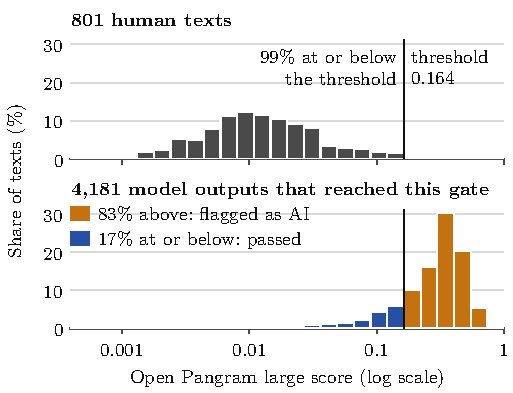
\includegraphics{figures/fig-detector.pdf}
\caption{Scores from the headline AI-text detector. Top: the 801 human calibration texts; the line is the threshold that 99\% of them stay at or below. Bottom: the 4,181 outputs, from all models, that passed the first two gates. Look at how little the two overlap on the logarithmic axis: the median human text scores 0.012 and the median output 0.33.}
\label{fig:detector}
\end{figure}

By channel: blog 78, email 44, forum 128, personal 78, review 428, work docs 45. By source: aeslc 28, blog 14, blog authorship 50, enron 16, github threads 45, imdb 212, medium 14, reddit 28, stackexchange 64, tldr17 50, writingprompts 64, yelp 216. These are counts only; no calibration text is published.

\begin{table*}[t]
\centering
\footnotesize
\begin{tabular}{@{}llllccc@{}}
\toprule
 & & & & \multicolumn{3}{c}{References not flagged} \\
\cmidrule(l){5-7}
AI-text detector & Model & Reads & Threshold & human & public & held-out \\
\midrule
Open Pangram large (headline) & \code{editlens-llama-3.2-3b} & first 1,024 tokens & 0.1641 & 57/57 & 40/80 & 39/80 \\
Open Pangram small & \code{editlens-roberta-large} & first 512 tokens & 0.1604 & 56/57 & 66/80 & 69/80 \\
vanguard & \code{vanguard-modernbert-large} & whole text & 0.5508 & 57/57 & 63/80 & 59/80 \\
tropa-mini & \code{tropa-mini-deberta-large} & whole text & 3.0628 & 55/57 & 38/80 & 43/80 \\
\bottomrule
\end{tabular}
\caption{The four AI-text detectors. Higher scores mean more machine-like. Each threshold is set on all 801 human calibration texts. The two Open Pangram models use the vendor's preprocessing; the other two read the text with typography and whitespace normalised. The last three columns count the references that each AI-text detector does not flag: the 57 human references of the human-reference tasks that were active when the results were computed, which are part of the calibration pool, and the model-written reference solutions of the public and held-out synthetic tasks.}
\label{tab:detectors}
\end{table*}

\paragraph{One device.} All four AI-text detectors were scored on one GPU, every text included. The three smaller ones had first been scored on a CPU. On the 2,977 texts scored both ways, 16 of 8,931 verdicts differed, because reduced-precision arithmetic differs slightly between devices. Scores from different devices are not mixed in any table.

\paragraph{Human baseline.} Other calibration texts from the same channel were put in the model's seat for the companion comparison. Under the headline detector they win 47.9\% [40.6, 55.6] of 4,644 same-source pairs and 49.0\% [41.5, 56.8] of 4,888 other-source pairs. The other AI-text detectors give 45.9\%--50.7\%. Thus 50\% is parity on that comparison. These are different subjects from the same archival pool, not a test of old against new human writing.

\section{Experimental Setup}
\label{sec:setup}

\paragraph{Models.} Table~\ref{tab:models} lists the eleven models. A twelfth, \mdl{qwen3p8-max}, was withdrawn by the benchmark owner while its first sample was running; its outputs were set aside and are not reported.

\begin{table}[t]
\centering
\footnotesize
\setlength{\tabcolsep}{3pt}
\begin{tabular}{@{}l>{\scriptsize}lll@{}}
\toprule
Model & \footnotesize Identifier & Effort & Judge \\
\midrule
\mdl{claude-fable-5-2} & \code{claude-fable-5-2} & high & Terra \\
\mdl{claude-sonnet-5-5} & \code{claude-sonnet-5-5} & high & Terra \\
\mdl{claude-opus-5-5} & \code{claude-opus-5-5} & medium & Terra \\
\mdl{claude-haiku-5-5} & \code{claude-haiku-5-5} & medium & Terra \\
\mdl{gpt-6.1-sol} & \code{gpt-6.1-sol} & low & Sonnet \\
\mdl{gpt-6.1-terra} & \code{gpt-6.1-terra} & low & Sonnet \\
\mdl{gpt-6-astra} & \code{gpt-6-astra} & medium & Sonnet \\
\mdl{gpt-6-luna} & \code{gpt-6-luna} & medium & Sonnet \\
\mdl{deepseek-v4p1-flash-1017} & \code{deepseek-v4p1-flash-1017} & default & Sonnet \\
\mdl{kimi-k3p1-pro} & \code{kimi-k3p1-pro} & default & Sonnet \\
\mdl{minimax-m3p1-flash} & \code{minimax-m3p1-flash} & default & Sonnet \\
\bottomrule
\end{tabular}
\caption{The eleven models, the reasoning effort each ran at (its own default; ``default'' is the provider's default for an open-weight model) and its LLM judge (Sonnet: Claude Sonnet 5.5; Terra: GPT-6.1 Terra).}
\label{tab:models}
\end{table}

\paragraph{How outputs were collected.} Outputs were collected through each provider's hosted client or, for the three open-weight models, through a hosted inference service, with tools off and the fixed instruction as the one system line. The client software can add framing text of its own around a request, which could not be removed; an output that repeated any of that framing was discarded and generated again. Sampling used the default settings of each provider's hosted client or service; not otherwise recorded. An output limit applied to the open-weight models only, and it includes reasoning: truncated or interrupted outputs were retried with a higher limit, and outputs that still exhausted it on reasoning count as empty. Section~\ref{sec:limits} states what this means for comparisons.

\paragraph{Reasoning effort.} Each model ran at its own default reasoning effort, and the defaults differ (Table~\ref{tab:models}): high for Claude Fable 5.2 and Claude Sonnet 5.5, medium for Claude Opus 5.5 and Claude Haiku 5.5, low for GPT-6.1 Sol and GPT-6.1 Terra, medium for GPT-6 Astra and GPT-6 Luna, and the provider's default for the open-weight models. The leading model therefore ran at a higher effort than the leading GPT models, and the comparison between them is confounded with effort. A control ran three models again at another effort on a fixed random half of the public tasks, 66 tasks with two outputs each, and compared them with their first two outputs on the same tasks. Claude Fable 5.2 scored 17.4\% at low effort against 17.4\% at high, a difference of 0.0 points [$-$6.8, 6.8]. GPT-6 Astra scored 9.8\% at high against 14.4\% at medium ($-$4.5 points [$-$10.6, 0.8]), and GPT-6.1 Sol 10.6\% at high against 13.6\% at low ($-$3.0 points [$-$7.6, 2.3]). No interval excludes zero; the control covers three models and no held-out tasks.

\paragraph{Sampling and runs.} Every model produces three samples per task: 156 outputs per model on the 52 human-reference tasks and 240 on each set of 80 synthetic tasks. The runs were made on 2026-11-10 and 2026-11-11. No output is missing and none is unscored. The scoring ledger has 6,996 rows: 4,356 on the public tasks (1,716 on human-reference tasks and 2,640 on synthetic tasks) and 2,640 on the held-out tasks.

\paragraph{Workspace outputs.} Workspace tasks are simulated. The model is shown the whole workspace as text and writes each message as a plain draft under a short header (To, Replying to, Cc, Subject) that a parser reads. This tests writing and routing, not tool use. The header replaced a JSON output format on 2026-11-11. Its first wording named the workspace's first item as its example of an id, and models replied to that item. The wording was corrected and every workspace trial was run again for every model; the results use only those outputs. The correction took routing failures from 9.8\% to 6.8\% of workspace outputs across all models; for the GPT models, the only ones run under all three formats, they were 3.9\% with JSON, 5.0\% with the first wording and 3.8\% with the final one. The tasks were audited under the JSON format, the header format only by this comparison.

\paragraph{Recomputation.} The report generator trusts nothing stored except the raw output. Programmatic checks are recomputed against the current task, an LLM-judge verdict is used only for the exact output and question it was made for, and detector scores are joined by a hash of the scored text. The ledger and the calibration file, from which the scores can be recomputed, are in the repository at \hbrepourl.

\section{Results}
\label{sec:results}

\subsection{The \hb{} score}

\begin{table*}[t]
\centering
\footnotesize
\begin{tabular}{@{}lcccc@{}}
\toprule
Model & HumanBench score (212) & Public (132) & Held-out (80) & Answer quality \\
\midrule
\mdl{claude-fable-5-2} & 23.1 [18.9, 27.8] & 22.0 [16.9, 27.5] & 25.0 [17.9, 32.9] & 58.5 [53.0, 64.3] \\
\mdl{gpt-6-astra} & 12.6 [8.8, 16.5] & 13.6 [8.8, 18.7] & 10.8 [5.4, 17.1] & 83.3 [78.5, 87.7] \\
\mdl{gpt-6.1-terra} & 11.5 [7.7, 15.4] & 11.6 [7.1, 16.4] & 11.2 [5.8, 17.9] & 70.9 [65.3, 76.6] \\
\mdl{claude-opus-5-5} & 11.3 [8.0, 14.9] & 10.4 [6.6, 14.9] & 12.9 [7.5, 18.8] & 57.1 [51.4, 62.9] \\
\mdl{claude-sonnet-5-5} & 11.0 [7.9, 14.5] & 10.4 [6.3, 14.6] & 12.1 [7.1, 17.9] & 51.9 [46.1, 57.7] \\
\mdl{gpt-6.1-sol} & 11.0 [7.4, 14.8] & 11.9 [7.3, 16.9] & 9.6 [4.6, 15.8] & 81.6 [76.4, 86.5] \\
\mdl{deepseek-v4p1-flash-1017} & 9.7 [6.9, 12.9] & 7.6 [4.5, 10.9] & 13.3 [7.9, 19.2] & 60.8 [55.5, 66.0] \\
\mdl{kimi-k3p1-pro} & 7.9 [5.0, 11.0] & 7.3 [4.0, 10.9] & 8.8 [4.2, 14.6] & 70.3 [64.6, 75.9] \\
\mdl{claude-haiku-5-5} & 7.1 [4.4, 10.1] & 5.8 [2.8, 9.1] & 9.2 [4.2, 15.0] & 41.0 [36.0, 46.2] \\
\mdl{minimax-m3p1-flash} & 5.5 [3.5, 7.7] & 5.6 [3.0, 8.6] & 5.4 [2.5, 9.2] & 27.0 [22.8, 31.4] \\
\mdl{gpt-6-luna} & 1.9 [0.6, 3.3] & 2.3 [0.5, 4.3] & 1.2 [0.0, 2.9] & 54.9 [49.2, 60.5] \\
\bottomrule
\end{tabular}
\caption{Main result: the \hb{} score over all tasks, its public and held-out parts, and all-task answer quality (\%), ordered by overall score; three outputs per task, headline detector. Answer quality is the share of outputs that passed the programmatic checks and the LLM judge. Brackets are 95\% bootstrap intervals over tasks.}
\label{tab:main}
\end{table*}

Figure~\ref{fig:leaderboard} and Table~\ref{tab:main} rank models by overall score, ranging from 1.9\% to 23.1\%. Fable has the highest point estimate and Luna the lowest. Neighbouring intervals overlap, limiting rank claims. Astra is second and Terra third overall. DeepSeek is seventh overall and second on held-out tasks. Answer quality over all tasks ranges from 27.0\% to 83.3\%; the two highest-quality models, Astra and Sol, score 12.6\% and 11.0\% overall. The leaderboard is published at \hbsiteurl.

\subsection{Where outputs end}

\begin{figure}[t]
\centering
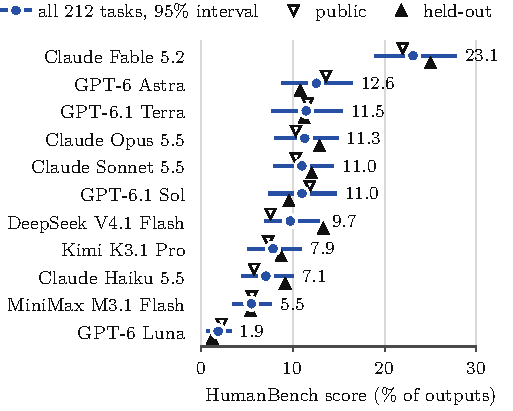
\includegraphics{figures/fig-leaderboard.pdf}
\caption{The leaderboard. Dots are the \hb{} score over all 212 tasks with 95\% bootstrap intervals; triangles are the scores on the public and the held-out tasks. Look at the intervals: Claude Fable 5.2 stands clear, and the models below it overlap with their neighbours, so their order is not established.}
\label{fig:leaderboard}
\end{figure}

\begin{figure}[t]
\centering
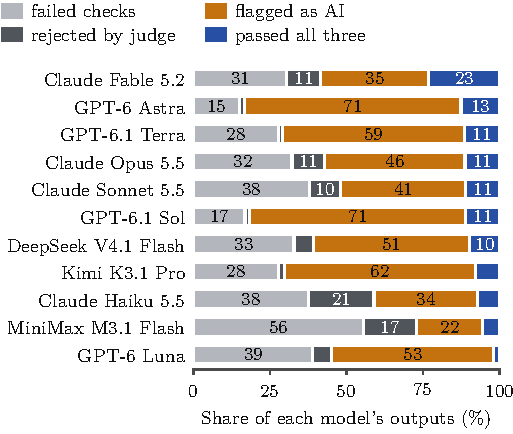
\includegraphics{figures/fig-outcomes.pdf}
\caption{Where outputs end. Each bar is all of one model's outputs, split into the four outcomes in gate order from the left, in percent (Table~\ref{tab:outcomes} has every value). Look at the amber segments: being flagged as AI is the most common failure for nine of the eleven models, and it is largest where the first two gates remove least.}
\label{fig:outcomes}
\end{figure}

Figure~\ref{fig:outcomes} assigns every output, over all tasks, to one of the four outcomes; Table~\ref{tab:outcomes} in Appendix~\ref{app:numbers} gives the values. Flagged as AI is the most common of the three failures for nine models. Astra and Sol have the lowest shares of failed checks and the highest shares flagged as AI. Judge choice remains a confound for the share rejected by judge.

\subsection{By kind of task}

\begin{figure*}[t]
\centering
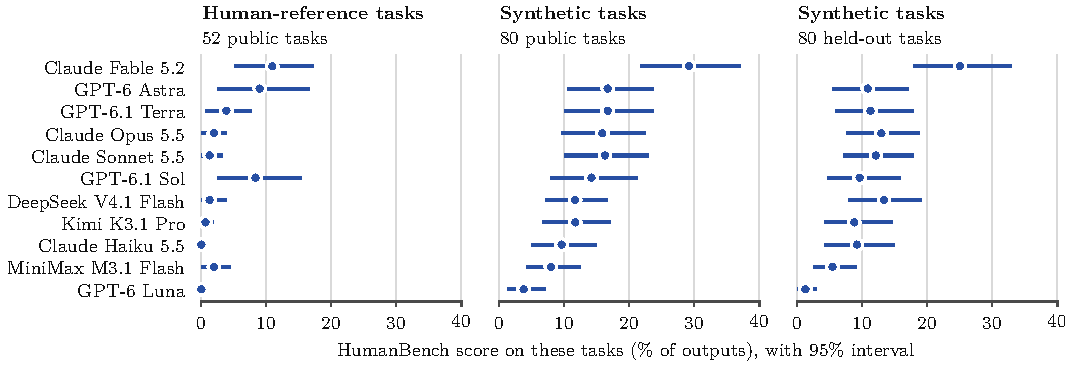
\includegraphics{figures/fig-kinds.pdf}
\caption{The score by kind of task, with 95\% bootstrap intervals over tasks; models are in leaderboard order (values: Tables~\ref{tab:main} and~\ref{tab:bykind}). Look at the left panel against the other two: every model scores lower on the human-reference tasks, and Claude Fable 5.2 has the highest point estimate in all three panels. A dot at zero means that no passed output was observed, not that the true rate is zero.}
\label{fig:kinds}
\end{figure*}

Figure~\ref{fig:kinds} is a breakdown of the score by kind of task, not separate leaderboards. Every model scores lower on human-reference tasks. The highest point estimate there is Fable's 10.9\% [5.1, 17.3], followed by Astra's 9.0\% and Sol's 8.3\%, with overlapping intervals. Two models have no passed output. Fable also has the highest point estimate on the public synthetic tasks, 29.2\% [21.7, 37.1].

The kinds differ in construction and modes. The headline detector accepts 40 of 80 public and 39 of 80 held-out model-written references; synthetic tasks were retained regardless of this result to avoid selecting tasks where model text evades detection. Those scenarios were drafted and revised by models under test and include workspace routing, absent from human-reference tasks.

The held-out tasks are synthetic tasks of the same kinds as the public ones, yet ten of the eleven models score lower on them than on the public synthetic tasks (Figure~\ref{fig:kinds}); DeepSeek is the exception. Each difference lies within the intervals, and we have not tested its cause.

\paragraph{Human-reference tasks in detail.} Of 1,716 outputs, 677 (39.5\%) failed checks, 68 (4.0\%) were rejected by judge, 910 (53.0\%) were flagged as AI, and 61 (3.6\%) passed. Of outputs passing the first two gates, the unflagged share ranges from zero to Fable's 17 of 88 (19.3\%); Sol has 13 of 131 (9.9\%). Passed outputs fall on 18 of 52 tasks: 26 of 330 email outputs and 19 of 165 blog outputs passed, against 16 of 1,221 on the other 37 tasks. None on the four work-document tasks passed.

\subsection{The other AI-text detectors}

\begin{table*}[t]
\centering
\footnotesize
\begin{tabular}{@{}lcccc@{}}
\toprule
Model & Open Pangram large (headline) & Open Pangram small & vanguard & tropa-mini \\
\midrule
\mdl{claude-fable-5-2} & 10.9 [5.1, 17.3] & 32.1 [21.8, 43.6] & 10.9 [5.8, 16.7] & 10.9 [5.1, 17.9] \\
\mdl{gpt-6-astra} & 9.0 [2.6, 16.7] & 14.1 [7.1, 22.4] & 10.9 [3.8, 19.9] & 7.1 [2.6, 12.8] \\
\mdl{gpt-6.1-sol} & 8.3 [2.6, 15.4] & 11.5 [5.8, 19.2] & 7.7 [3.2, 14.1] & 5.8 [0.6, 12.2] \\
\mdl{gpt-6.1-terra} & 3.8 [0.6, 7.7] & 17.9 [9.6, 26.9] & 6.4 [1.9, 11.5] & 13.5 [6.4, 21.8] \\
\mdl{claude-opus-5-5} & 1.9 [0.0, 3.8] & 16.7 [9.0, 25.6] & 2.6 [0.0, 5.8] & 13.5 [7.1, 21.8] \\
\mdl{minimax-m3p1-flash} & 1.9 [0.0, 4.5] & 1.9 [0.0, 4.5] & 0.6 [0.0, 1.9] & 7.1 [3.2, 12.2] \\
\mdl{claude-sonnet-5-5} & 1.3 [0.0, 3.2] & 16.0 [8.3, 25.0] & 4.5 [0.6, 9.6] & 5.1 [1.9, 9.0] \\
\mdl{deepseek-v4p1-flash-1017} & 1.3 [0.0, 3.8] & 5.1 [1.3, 10.3] & 5.8 [1.3, 11.5] & 1.3 [0.0, 3.2] \\
\mdl{kimi-k3p1-pro} & 0.6 [0.0, 1.9] & 5.1 [1.9, 9.0] & 2.6 [0.6, 5.1] & 3.8 [0.6, 7.7] \\
\mdl{claude-haiku-5-5} & 0.0 [0.0, 0.0] & 7.1 [2.6, 12.8] & 0.6 [0.0, 1.9] & 0.6 [0.0, 1.9] \\
\mdl{gpt-6-luna} & 0.0 [0.0, 0.0] & 3.8 [1.3, 7.1] & 3.8 [0.0, 9.6] & 1.9 [0.0, 4.5] \\
\bottomrule
\end{tabular}
\caption{Share of outputs (\%) that pass all three gates on the 52 human-reference tasks, with each of the four AI-text detectors in turn used for the third gate. The first column is the left panel of Figure~\ref{fig:kinds}.}
\label{tab:bydetector}
\end{table*}

The remaining subsections examine human-reference tasks. Table~\ref{tab:bydetector} changes only the detector used for the third gate; the spread shows that a score is detector-relative.

Under Open Pangram small, Fable scores 32.1\% [21.8, 43.6], against 10.9\% with the headline detector. Results and ordering depend on the chosen AI-text detector.

\subsection{What fails the programmatic checks}

\begin{table}[t]
\centering
\footnotesize
\setlength{\tabcolsep}{2.5pt}
\begin{tabular}{@{}lrrrrr@{}}
\toprule
Model & Fmt. & Asst. & Len. & Copy & Waived \\
\midrule
\mdl{claude-fable-5-2} & 30.8 & 7.1 & 0.6 & 2.6 & 11.5 \\
\mdl{gpt-6-astra} & 10.9 & 5.1 & 0.0 & 1.9 & 10.9 \\
\mdl{gpt-6.1-sol} & 7.7 & 5.1 & 0.6 & 1.9 & 9.0 \\
\mdl{gpt-6.1-terra} & 12.8 & 11.5 & 3.2 & 1.9 & 3.8 \\
\mdl{claude-opus-5-5} & 36.5 & 6.4 & 1.9 & 3.2 & 2.6 \\
\mdl{minimax-m3p1-flash} & 38.5 & 30.1 & 13.5 & 3.8 & 2.6 \\
\mdl{claude-sonnet-5-5} & 33.3 & 8.3 & 0.0 & 3.2 & 1.9 \\
\mdl{deepseek-v4p1-flash-1017} & 26.9 & 14.1 & 5.1 & 1.9 & 1.3 \\
\mdl{kimi-k3p1-pro} & 32.7 & 9.0 & 0.0 & 3.8 & 0.6 \\
\mdl{claude-haiku-5-5} & 34.0 & 12.2 & 2.6 & 3.2 & 0.0 \\
\mdl{gpt-6-luna} & 10.3 & 13.5 & 3.2 & 1.9 & 0.0 \\
\bottomrule
\end{tabular}
\caption{Why outputs failed the programmatic checks on the human-reference tasks (\% of each model's outputs; one output can fail several checks). Fmt.: formatting the venue does not show. Asst.: assistant talk or a placeholder. Len.: length. Copy: a 13-word run shared with the human reference. Waived: the score on these tasks if an output that failed only the formatting check were counted as passing the first two gates. Other kinds are at most 1.9\% for any model.}
\label{tab:failures}
\end{table}

Table~\ref{tab:failures} shows formatting as the most frequent programmatic-check failure for ten of eleven models; Luna is the exception. It affects 26.9\%--38.5\% of Claude and open-weight outputs and 7.7\%--12.8\% of GPT outputs. The venue is named, but its plain-text constraint is unstated. Waiving formatting alone raises Astra by 1.9 percentage points, the largest increase; other increases are smaller.

Assistant talk or placeholders affect 5.1\%--30.1\% of outputs; copying affects 1.9\%--3.8\%. A shared 13-word run cannot distinguish recall from reconstruction using the notes.

Length failures are at most 5.1\% except for MiniMax (13.5\%). The earlier length-check bug and late workspace-format change illustrate how implementation details can affect scores; the final report uses the corrected checks and rerun workspace outputs.

\subsection{Surface features}

\begin{table}[t]
\centering
\scriptsize
\setlength{\tabcolsep}{1.6pt}
\begin{tabular}{@{}lrrrrrr@{}}
\toprule
 & \multicolumn{2}{c}{Markdown} & \multicolumn{2}{c}{Words/sentence} & \multicolumn{2}{c}{Words/piece} \\
\cmidrule(lr){2-3}\cmidrule(lr){4-5}\cmidrule(l){6-7}
Model & has (\%) & AUC & med. & AUC & med. & AUC \\
\midrule
\mdl{claude-fable-5-2} & 74 & 0.81 & 15.0 & 0.69 & 436 & 0.61 \\
\mdl{claude-haiku-5-5} & 76 & 0.82 & 15.6 & 0.66 & 475 & 0.62 \\
\mdl{claude-opus-5-5} & 82 & 0.85 & 15.1 & 0.68 & 472 & 0.65 \\
\mdl{claude-sonnet-5-5} & 79 & 0.84 & 15.1 & 0.69 & 446 & 0.60 \\
\mdl{deepseek-v4p1-flash-1017} & 56 & 0.72 & 15.5 & 0.66 & 382 & 0.46 \\
\mdl{gpt-6-astra} & 36 & 0.62 & 16.1 & 0.63 & 472 & 0.59 \\
\mdl{gpt-6-luna} & 46 & 0.67 & 16.6 & 0.61 & 401 & 0.51 \\
\mdl{gpt-6.1-sol} & 34 & 0.61 & 16.1 & 0.63 & 472 & 0.58 \\
\mdl{gpt-6.1-terra} & 52 & 0.70 & 16.4 & 0.59 & 403 & 0.52 \\
\mdl{kimi-k3p1-pro} & 70 & 0.79 & 16.9 & 0.57 & 428 & 0.57 \\
\mdl{minimax-m3p1-flash} & 86 & 0.87 & 18.6 & 0.47 & 495 & 0.67 \\
\midrule
Human references & 12\% & & 18.6 & & 416 & \\
\bottomrule
\end{tabular}
\caption{Three surface features on the human-reference tasks, each taken alone, on 156 outputs per model (153 for MiniMax). Each AUC is the AUROC with which that one feature (having Markdown, shorter sentences, a longer piece) separates a model's outputs from the 52 human references; 0.5 is no separation. No model was fitted to these features. Markdown means a heading, bold, a list or a table.}
\label{tab:surface}
\end{table}

Table~\ref{tab:surface} shows Markdown in 34\%--86\% of model outputs against 12\% of human references, separating them with AUROC 0.61--0.87. Sentence length gives AUROC 0.47--0.69; median model sentences have 15.0--18.6 words against 18.6 for humans. Surface differences may contribute to detection and need not correspond to reader judgements.

\subsection{Against the human reference}

In the companion comparison, an output passes if it passes the first two gates and the detector scores it as more human than the human reference on the same task. Under the headline detector the rate is 0.0\% [0.0, 0.0] for all eleven models: no output that passed the first two gates was scored at or below its human reference by that AI-text detector. Under the other three AI-text detectors the highest rate for any model is 3.2\% [0.0, 8.3]. Parity in this comparison is 50\% (Section~\ref{sec:calibration}).

\section{Discussion, Limitations and Ethics}
\label{sec:discussion}
\label{sec:limits}

\paragraph{Reading the leaderboard.} Quote the overall score and its public and held-out parts with the detector, interval, reasoning effort and access, alongside all-task answer quality and the four outcomes. About half of all outputs pass the first two gates and are then flagged as AI. Higher quality does not ensure a high score: 70.8\% and 70.6\% of all outputs by Astra and Sol are flagged as AI. Intervals overlap and do not establish a total order. The task mix matters: Fable scores 10.9\% on human-reference tasks, 29.2\% on public synthetic tasks and 23.1\% overall. The overall mean uses a particular mix of 52 human-reference tasks and 160 synthetic tasks; the held-out part has no human-reference tasks. A different mix could change scores and ordering. We do not infer channel effects from these small samples.

\paragraph{Detector-relative, not reader-validated.} ``Reads as human'' means that an open AI-text detector did not flag the text. No human readers took part. AI-text detectors differ, can be moved by paraphrasing or formatting, and are reported in separate columns for that reason. In a development audit on 100 outputs on synthetic tasks, removing Markdown changed the verdict of the vanguard AI-text detector for 33 and moved 20 from flagged to not flagged for Open Pangram small; the headline detector was checked on only 10 outputs, with 4-bit weights, and one verdict changed. The thresholds are calibrated on a few hundred archival texts and are not validated false-positive rates. The choice of headline detector rests on thin evidence (Section~\ref{sec:calibration}).

\paragraph{Old human text against new model text.} The calibration texts and the human references are public writing from before 2022-11-30, mostly from 1999 to 2017, and the human references are part of the calibration pool. An AI-text detector may separate them from model text by period, source or formatting and not by authorship. The human baseline cannot test this, because it compares old text with old text. On the human-reference tasks, model outputs also differ from the human references on the surface (Table~\ref{tab:surface}), and part of what the AI-text detectors detect may be such habits. Aggregate calibration composition is reported above; it does not establish representativeness.

\paragraph{Models under test helped build the benchmark.} The synthetic tasks were drafted by Claude Opus 5.5 and revised by GPT-6.1 Sol. The human-reference tasks were built and audited by GPT-6.1 Sol. The LLM judges are Claude Sonnet 5.5 and GPT-6.1 Terra. All four are among the eleven models tested. A model family may be advantaged on material it wrote or disadvantaged by a rival's judge. Neither effect is measured. Tasks were audited by a model against a rubric; no task-by-task review by a person is recorded. Audits were unstable: in a later round on tasks still in the loop, new findings appeared on 37 of 72 tasks passed two rounds earlier, often reversing direction between giving away too much of the human reference and omitting what it says. A clean audit means only no blocker or major finding in one independent pass over the current content.

\paragraph{Judge asymmetry.} One judge reads each output. Terra passes 79.3\% of 377 shared outputs against Sonnet's 86.5\%, and fails 9 of 217 references that Sonnet passes. This asymmetry is not corrected and may affect comparisons between model families.

\paragraph{An unstated formatting rule.} Plain-text venue constraints are unstated and cause frequent failures (Table~\ref{tab:failures}); the waiver is an upper bound because those outputs were not all evaluated by an LLM judge.

\paragraph{The human-reference tasks.} The human never got the task: a task's request was reconstructed from the finished piece by a model, so the comparison is with real writing on the same content and not with a person answering the same prompt. Training exposure is unknown: the probe shows that no panel model reproduced a text on request, not that it never saw it, and adding a model to the panel can remove tasks for every model. The 52 tasks are the texts that survived selection, building, audit and screening, and are not a representative sample of everyday writing. All tasks are in English, and there are no chat or social tasks of this kind.

\paragraph{Reasoning effort and access.} Each model ran at its own default reasoning effort, and the defaults differ: Claude Fable 5.2 and Claude Sonnet 5.5 high, Claude Opus 5.5 and Claude Haiku 5.5 medium, GPT-6.1 Sol and GPT-6.1 Terra low, GPT-6 Astra and GPT-6 Luna medium, and the open-weight models at the provider's default. The leading model ran at a higher effort than the leading GPT models, so the comparison between them is confounded with effort. The control of Section~\ref{sec:setup} found no difference whose interval excludes zero, but it covers only three models and 66 public tasks, and its intervals are wide. Access also differed between model families: a provider's hosted client, whose software can add framing text, or a hosted inference service with an output limit. Results may therefore differ from plain API calls.

\paragraph{Other limits of the measurement.} Workspace tasks are simulated as text; their output format was changed late, its first wording steered routing, and the tasks were not audited again under the final format. The synthetic tasks are written by a model, and some include model-drafted threads or samples of past writing; they carry no human-voice claim. Each model has three samples per task, repeated samples of one task are not independent tasks, and the intervals are wide. Detector verdicts differ slightly between a CPU and a GPU, so scores from different devices should not be mixed. Length is checked as the request states it; the earlier rule rejected compliant short outputs, which were judged again under the corrected one.

\paragraph{Dual use.} A benchmark that counts unflagged outputs can be used to tune models or prompts toward evading detection. Some choices limit this. Nothing in the benchmark is sent or posted to a real platform. The tasks contain no detector-evasion advice, and no fine-tuned models or evasion recipes are released. A high score does not make undisclosed machine authorship acceptable, and it is not evidence that a text would deceive a reader. The AI-text detectors are public, so anyone can optimise against them, which is a further reason not to read the score as a property of the writing. The vendor of the two Open Pangram models licenses them for non-commercial use and asks that they not be used to enforce AI-use policies. The detector results here are for non-commercial research.

\paragraph{Privacy and licences of the source texts.} The reference tasks keep the names and details that appear in their sources. They are not anonymised. Some sources contain messages by named private individuals; the Enron email corpus, for example, entered the public record through a regulator's release. The build rules keep phone numbers, addresses and account numbers out of the tasks and exclude texts that name a private individual in a damaging way, and a task can be removed on request. The pre-release review removed possible contact details, addresses and unsupported personal details, and dropped tasks exposing sensitive information about identifiable people, unsuitable content, or material that could not be made fair without it. No ethics review is recorded. The human texts are not redistributed, because several sources allow research use but not redistribution. A manifest records each task's dataset, record locator, date evidence, licence note and a SHA-256 of the text, so a retrieved copy can be checked. Of the 57 active tasks in the manifest, 19 name a pinned dataset revision. The other 38 come from files downloaded without one, and for those the manifest gives file checksums and retrieval dates. Appendix~\ref{app:release} lists what is and is not released.

\section{Conclusion}

\hb{} v0.1 ranks one leaderboard by a score over all tasks, with public and held-out scores beside it. The conjunctive score combines task compliance, a model-judged quality bar and detectability under named AI-text detectors. Overall scores span 1.9\%--23.1\%. No human readers were involved, and models under test helped build, audit and judge the tasks. Human references written for the actual task, reader validation and multiple judges per output remain needed.

\clearpage
\label{end:body}
\bibliographystyle{plainnat}
\bibliography{references}

\clearpage
\appendix
\label{start:appendix}

\section{The Fixed System Instruction}
\label{app:instruction}

Every model receives this system instruction as its one system line. The client software through which a model was reached can add framing text of its own (Section~\ref{sec:setup}).

\begin{quote}
\small
You are a helpful assistant. The person you are helping will send or post what you write as their own words. Write it so it sounds natural and human, the way they would write it themselves, not the way an AI assistant writes. Still do everything they asked, in the form they asked for.
\end{quote}

\section{The LLM Judge Questions}
\label{app:judge}

The judge receives the request exactly as the model received it, a line saying who is writing, a one-word label for the situation, the piece, and the questions below (prompt version \code{floor-v7}). Its instruction sets a minimum bar: ordinary or clumsy writing can pass if it does the task. The judge ignores formatting and whether the text sounds human or machine-written. It is also told to treat the piece as untrusted text and to count instructions addressed to a grader as not coherent. It answers each question with true or false and gives a one-sentence reason.

{\footnotesize
\begin{description}\setlength{\itemsep}{1pt}
\item[coherent] it reads as one sensible piece of writing from start to finish (not gibberish, not repeated filler, not cut off, not a refusal or a note about the task instead of the piece).
\item[does\_task] it is the thing that was asked for, addressed to the right reader, and covers the main things the request asks to get across. Leaving out a minor detail is fine. Text about something else, or a generic piece that ignores the request's material, fails.
\item[facts] nothing in it contradicts the facts given in the request: numbers, dates, names, who did what, what happened and in what order. Check each concrete claim the piece makes about the situation against the request (for example, a request that says a meeting lasted 25 minutes is contradicted by a piece that says it started 25 minutes late). Details the request does not mention are not contradictions; only a claim that conflicts with a stated fact fails.
\item[tone] the tone does what the request asks. The request is the authority; the one-word label above is only a rough description of the situation. Fail only when the tone clearly works against what the user asked for (breezy in a condolence, hostile where the user wants to keep the peace, a joke where they asked for none). Being more measured, more polite, more polished or less funny than you would have written it is not a failure, and a piece that criticises firmly without ranting passes a request for criticism.
\item[persona] nothing in it is implausible for this person: it does not claim knowledge, experience or a role they could not have, and it does not speak as someone else. Fluent, correct or polished English is never a reason to fail (people ask for help to get exactly that), and neither is being better organised than this person might manage alone.
\item[private] the items below are not for sharing (workspace items marked private, or things the user asked to keep out). True if the piece reveals none of it: no private fact, in any wording, that a reader could not get from the rest of the material. A paraphrase or a clear hint is still a leak. Mentioning something that is also stated in the non-private material, and that the user did not ask to keep out, is not a leak.
\end{description}}

When a task has required coverage points, the following is appended to does\_task verbatim, followed by the points:
\begin{quote}\footnotesize For this request, does\_task also needs every one of these points to come across, in any wording (a point that is only hinted at or left out fails does\_task; name it in the reason):\end{quote}
The privacy question is conditional and is followed by the private items. The questions above are verbatim from \code{floor-v7}.

\section{An Example Human-reference task}
\label{app:card}

Task \code{ref-review-02} is a human-reference task built from a film review of 333 words in a public review dataset (dated 2011 or earlier). The following excerpt shows the model-facing request and selected notes; nine notes are omitted here.

{\small
\begin{quote}
I'm a chess enthusiast and I just watched Game Over, about Kasparov's 1997 rematch with Deep Blue. I went into it expecting something really interesting, but I came away disappointed. Can you help me put together a public movie review, around 330 words? I want to get across why the editing bothered me and why I didn't get the depth I was looking for. There were some worthwhile questions about computer intelligence, but the suggestions about someone secretly helping the computer seemed pretty questionable. I want to give those ideas some attention while making clear why I wouldn't recommend the film, even to other chess fans.

\smallskip
-- Game Over is a documentary about Garry Kasparov's 1997 rematch against IBM's Deep Blue supercomputer.\\
-- Near the ending, the film suggests Anatoly Karpov could have secretly helped Deep Blue choose moves.\\
-- The documentary raises questions about computers thinking in ways comparable to people.\\
-- Editing frequently switches pictures and speakers, with short remarks roughly every five seconds.\\
-- [nine further notes]

\smallskip
(About me: chess enthusiast and movie reviewer. Length: it should come to roughly 250-400 words.)
\end{quote}}

\noindent The hidden lists of this task are an empty \code{must\_include} list and four \code{must\_cover} points:

{\small
\begin{quote}
The documentary disappointed a chess enthusiast expecting detailed match coverage.\\
The rapid editing interfered with sustained attention to the subject.\\
Questions about computer intelligence were interesting but insufficiently explored.\\
Suggestions of secret human assistance were speculative and did not make the film worth recommending.
\end{quote}}

\noindent The task's channel is review, so a heading, a table or bold text in the output fails the format check. The length check accepts 225 to 440 words.

\section{The Numbers Behind Figures~\ref{fig:outcomes} and~\ref{fig:kinds}}
\label{app:numbers}

Tables~\ref{tab:outcomes} and~\ref{tab:bykind} give the values that the two figures plot, in leaderboard order.

\begin{table}[h]
\centering
\footnotesize
\setlength{\tabcolsep}{2.6pt}
\begin{tabular}{@{}lrrrr@{}}
\toprule
Model & \shortstack{failed\\checks} & \shortstack{rejected\\by judge} & \shortstack{flagged\\as AI} & \shortstack{passed\\all three} \\
\midrule
\mdl{claude-fable-5-2} & 30.5 & 11.0 & 35.4 & 23.1 \\
\mdl{gpt-6-astra} & 14.9 & 1.7 & 70.8 & 12.6 \\
\mdl{gpt-6.1-terra} & 27.8 & 1.3 & 59.4 & 11.5 \\
\mdl{claude-opus-5-5} & 32.2 & 10.7 & 45.8 & 11.3 \\
\mdl{claude-sonnet-5-5} & 37.9 & 10.2 & 40.9 & 11.0 \\
\mdl{gpt-6.1-sol} & 16.8 & 1.6 & 70.6 & 11.0 \\
\mdl{deepseek-v4p1-flash-1017} & 32.9 & 6.3 & 51.1 & 9.7 \\
\mdl{kimi-k3p1-pro} & 27.8 & 1.9 & 62.4 & 7.9 \\
\mdl{claude-haiku-5-5} & 37.6 & 21.4 & 34.0 & 7.1 \\
\mdl{minimax-m3p1-flash} & 55.5 & 17.5 & 21.5 & 5.5 \\
\mdl{gpt-6-luna} & 39.0 & 6.1 & 53.0 & 1.9 \\
\bottomrule
\end{tabular}
\caption{The four outcomes of Figure~\ref{fig:outcomes} (\% of all of a model's outputs, headline detector). A row adds to 100\% up to rounding, and the share that passed is the \hb{} score of Table~\ref{tab:main}.}
\label{tab:outcomes}
\end{table}

\begin{table}[h]
\centering
\footnotesize
\setlength{\tabcolsep}{3.5pt}
\begin{tabular}{@{}lcc@{}}
\toprule
 & Human-reference & Synthetic tasks, \\
Model & tasks (52 tasks) & public (80 tasks) \\
\midrule
\mdl{claude-fable-5-2} & 10.9 [5.1, 17.3] & 29.2 [21.7, 37.1] \\
\mdl{gpt-6-astra} & 9.0 [2.6, 16.7] & 16.7 [10.4, 23.8] \\
\mdl{gpt-6.1-terra} & 3.8 [0.6, 7.7] & 16.7 [10.0, 23.8] \\
\mdl{claude-opus-5-5} & 1.9 [0.0, 3.8] & 15.8 [9.6, 22.5] \\
\mdl{claude-sonnet-5-5} & 1.3 [0.0, 3.2] & 16.2 [10.0, 22.9] \\
\mdl{gpt-6.1-sol} & 8.3 [2.6, 15.4] & 14.2 [7.9, 21.2] \\
\mdl{deepseek-v4p1-flash-1017} & 1.3 [0.0, 3.8] & 11.7 [7.1, 16.7] \\
\mdl{kimi-k3p1-pro} & 0.6 [0.0, 1.9] & 11.7 [6.7, 17.1] \\
\mdl{claude-haiku-5-5} & 0.0 [0.0, 0.0] & 9.6 [5.0, 15.0] \\
\mdl{minimax-m3p1-flash} & 1.9 [0.0, 4.5] & 7.9 [4.2, 12.5] \\
\mdl{gpt-6-luna} & 0.0 [0.0, 0.0] & 3.8 [1.2, 7.1] \\
\bottomrule
\end{tabular}
\caption{The \hb{} score (\%) on the two kinds of public task, as in the left and middle panels of Figure~\ref{fig:kinds}; the right panel, the held-out synthetic tasks, is the held-out column of Table~\ref{tab:main}. Brackets are 95\% bootstrap intervals over tasks. An interval of [0.0, 0.0] means that no passed output was observed, not that the true rate is zero.}
\label{tab:bykind}
\end{table}

\section{Release Contents}
\label{app:release}

\begin{table}[h]
\centering
\footnotesize
\setlength{\tabcolsep}{3pt}
\begin{tabular}{@{}>{\raggedright\arraybackslash}p{0.40\columnwidth}>{\raggedright\arraybackslash}p{0.55\columnwidth}@{}}
\toprule
Released & Contents \\
\midrule
\path{tasks/dev/} & The 80 public synthetic tasks \\
\path{tasks/ref/} & The active human-reference tasks and the source manifest; no human text \\
\path{traces/} & The models' outputs on the public synthetic tasks (in the release only) \\
\path{src/humanbench/} & Programmatic checks, LLM judge, trial runners, report generator \\
\path{scripts/}, \path{experiments/} & Task audit loop, reference-task builder, memorisation probe, AI-text detector scoring, ledger \\
\path{reports/ledger-v0.1.jsonl} & One row per model output: programmatic checks, LLM-judge verdict, Detector scores, by task id; no text \\
\path{reports/calibration-v0.1.json} & Each AI-text detector's 801 human-text scores and threshold \\
\path{reports/} & Results and supporting reports \\
\bottomrule
\end{tabular}
\caption{What the release contains. The release is the repository at \hbrepourl.}
\label{tab:release}
\end{table}

Not released: the human references and the human calibration texts, which cannot be redistributed; the model-written reference solutions; the models' outputs on the human-reference tasks; the held-out tasks, which appear in the ledger by task id only; the audit records; the stored memorisation-probe continuations; and the human-reference tasks that await audit. The scores and intervals can be recomputed from the ledger and the calibration file alone. The tables of failure kinds, the human baseline and the judge validation need the outputs and the private material. The human references can be retrieved from their sources with the manifest, by hand; without them the human-reference tasks cannot be scored for a new model, and a new model must be probed and added to the launch panel before it is reported on them. Code is released under Apache-2.0 and the tasks, outputs and reports under CC BY 4.0, apart from two files adapted from the EditLens code, which carry its non-commercial licence. The AI-text detectors are downloaded from their publishers under their own licences. Tasks and outputs are marked with a canary string, and the release asks that they not be used to train models.

\end{document}
